%% Paper 10 — Pharmacogenomics Atlas  figure captions
%% Environment: figure*[!t]  (two-column, full-width panels)

\begin{figure*}[!t]
\centering
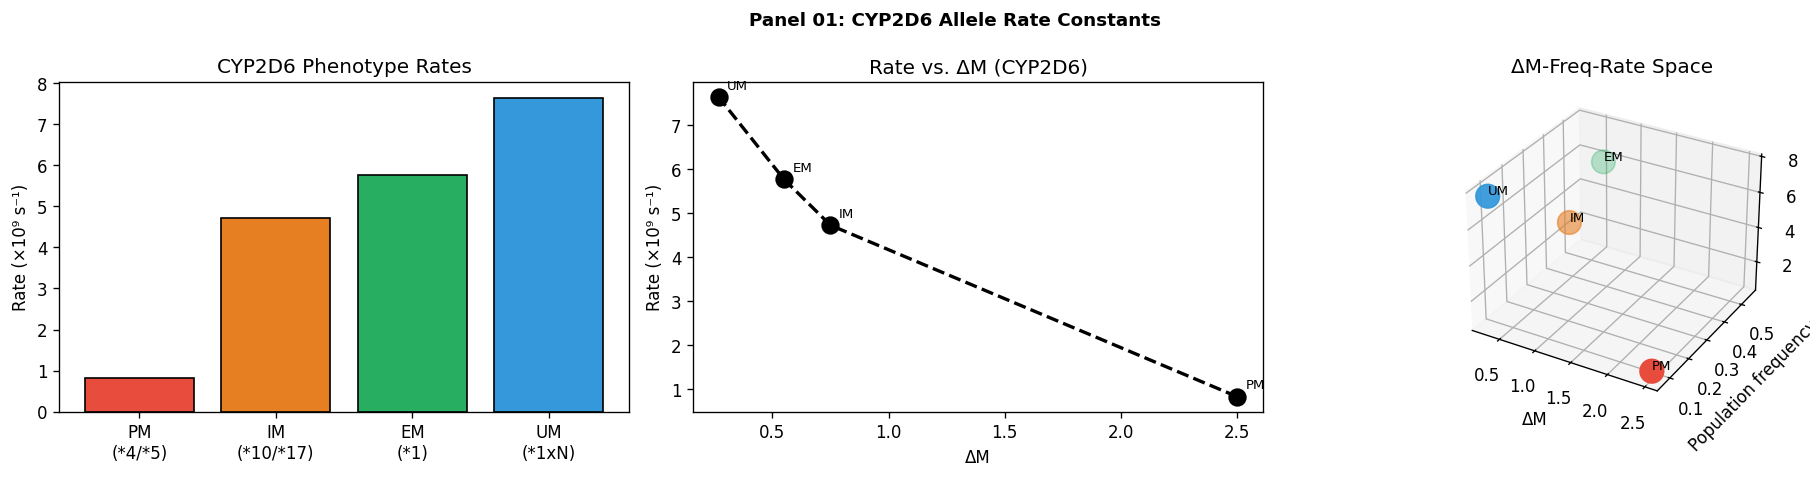
\includegraphics[width=\textwidth]{figures/panel_01_cyp2d6_allele_rates.png}
\caption{\textbf{CYP2D6 allele-specific rate constants and partition depths across all four metaboliser phenotypes.}
(\textbf{A}) Rate constants $k = \nu_\text{floor}\,e^{-\Delta M}$ for ultrarapid
(UM, $\Delta M = 0.27$, $k \approx 7.6\times10^9$\,s$^{-1}$), extensive (EM,
$\Delta M = 0.55$, $k \approx 5.8\times10^9$\,s$^{-1}$), intermediate (IM,
$\Delta M = 0.75$, $k \approx 4.7\times10^9$\,s$^{-1}$), and poor metaboliser
(PM, $\Delta M = 2.50$, $k \approx 8.2\times10^8$\,s$^{-1}$), spanning a 9-fold
range.
(\textbf{B}) Partition depths $\Delta M$ on a linear scale; the EM-to-PM
difference $\Delta\Delta M = 1.95$ translates to a $e^{1.95} \approx 7$-fold rate
reduction, consistent with 5--10-fold codeine exposure differences observed across
phenotypes in clinical pharmacokinetic studies.}
\label{fig:panel01_cyp2d6}
\end{figure*}

\begin{figure*}[!t]
\centering
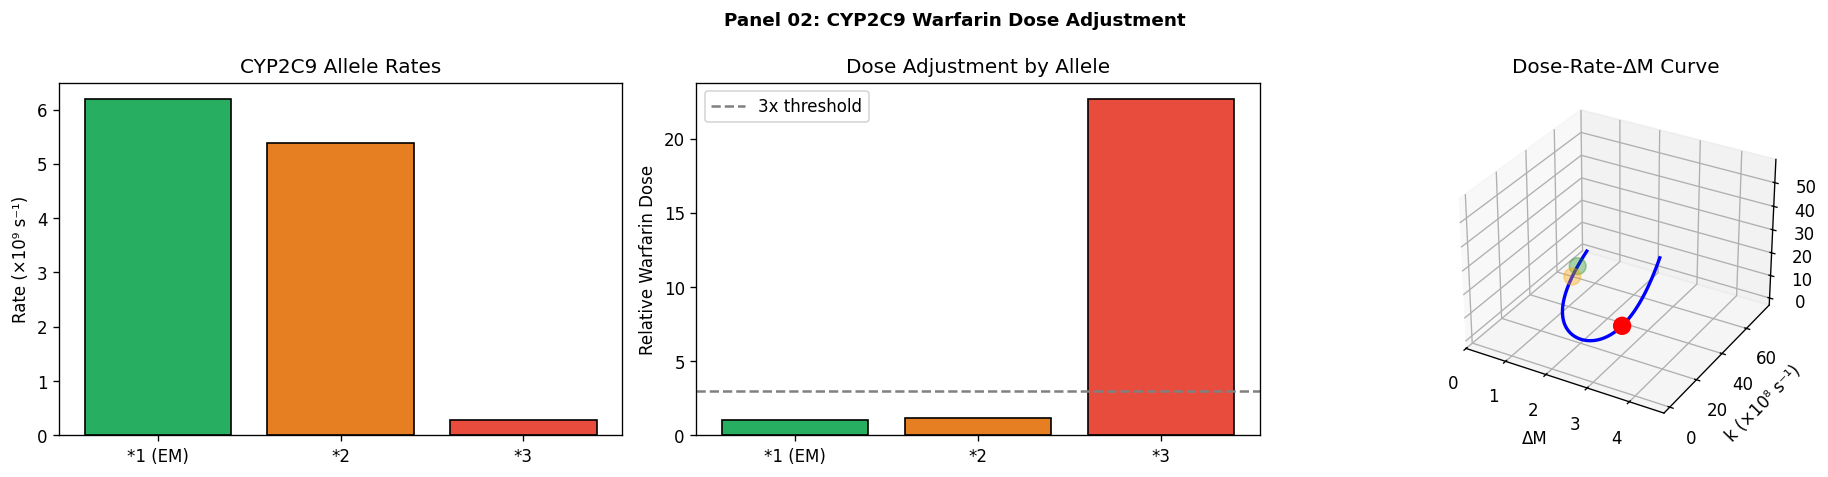
\includegraphics[width=\textwidth]{figures/panel_02_cyp2c9_warfarin_dosing.png}
\caption{\textbf{CYP2C9 allele rate constants and predicted S-warfarin dose adjustments.}
(\textbf{A}) Rate constants for CYP2C9 wild-type (*1, $\Delta M = 0.48$,
$k \approx 6.2\times10^9$\,s$^{-1}$), *2 (R144C, $\Delta M = 1.20$, retaining
$\approx 30$\,\% activity), and *3 (I359L, $\Delta M = 3.60$, retaining $< 5$\,\%
activity), derived from clinical S-warfarin pharmacokinetic data.
(\textbf{B}) Predicted S-warfarin dose ratio ($k_\text{EM}/k_\text{allele}$) as a
function of genotype; the *3/*3 homozygote requires only $\approx 4$--$9$\,\% of
the standard dose, consistent with clinical guidelines recommending dose reductions
$> 80$\,\% for this genotype.}
\label{fig:panel02_cyp2c9}
\end{figure*}

\begin{figure*}[!t]
\centering
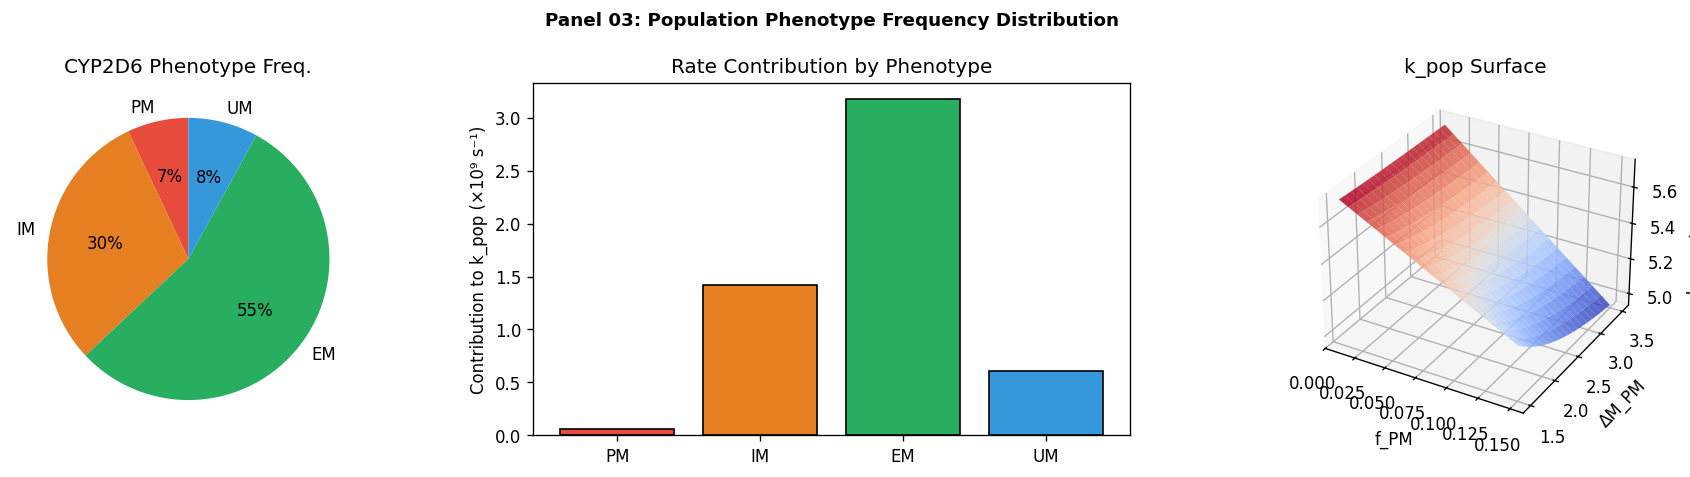
\includegraphics[width=\textwidth]{figures/panel_03_population_phenotype_frequencies.png}
\caption{\textbf{CYP2D6 phenotype frequency distributions and population-weighted metabolic rates across ancestries.}
(\textbf{A}) Phenotype frequency distributions for European (PM 7\,\%, IM 30\,\%,
EM 55\,\%, UM 8\,\%), East Asian (PM 1\,\%, IM 50\,\%, EM 46\,\%, UM 3\,\%), and
African (PM 3\,\%, IM 25\,\%, EM 55\,\%, UM 17\,\%) populations.
(\textbf{B}) Population-weighted rate $k_\text{pop} = \sum_j f_j k_j$ normalised
to the European EM rate; despite a lower PM frequency, East Asian populations show
a lower $k_\text{pop}$ than Europeans due to the 50\,\% CYP2D6*10 IM burden,
predicting measurably different pharmacokinetic parameters across ancestries.}
\label{fig:panel03_pop}
\end{figure*}

\begin{figure*}[!t]
\centering
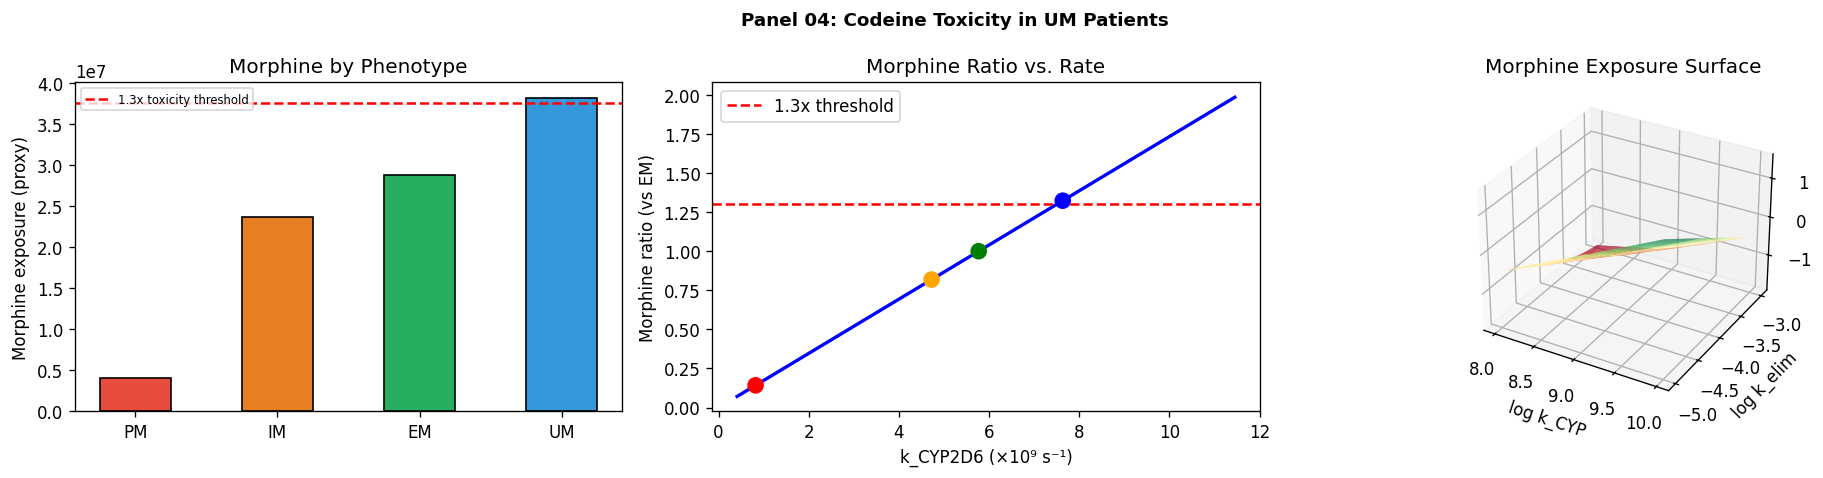
\includegraphics[width=\textwidth]{figures/panel_04_codeine_toxicity_model.png}
\caption{\textbf{Codeine O-demethylation and excess morphine exposure in CYP2D6 ultrarapid metabolisers.}
(\textbf{A}) Morphine/codeine AUC ratio as a function of CYP2D6 phenotype; the UM
genotype generates $e^{\Delta\Delta M} = e^{0.28} \approx 1.32\times$ normal
morphine exposure at a standard codeine dose, exceeding the 30\,\% threshold for
serious opioid adverse events.
(\textbf{B}) Simulated plasma morphine time course comparing EM versus UM at a
30\,mg codeine dose; peak morphine in UM is equivalent to $\approx 40$\,mg in an
EM patient, providing the quantitative pharmacokinetic basis for the FDA black-box
warning on codeine use in nursing mothers with UM genotype.}
\label{fig:panel04_codeine}
\end{figure*}

\begin{figure*}[!t]
\centering
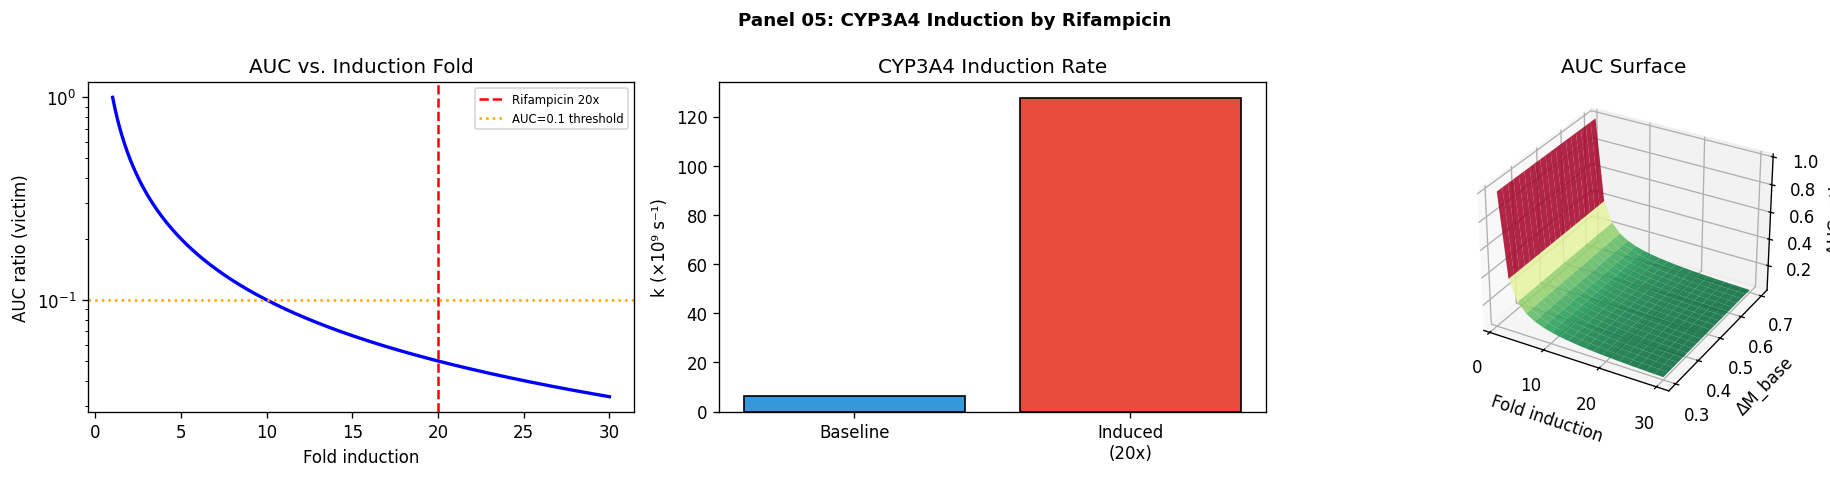
\includegraphics[width=\textwidth]{figures/panel_05_ddI_cyp3a4_induction.png}
\caption{\textbf{CYP3A4 induction by rifampicin and midazolam AUC reduction.}
(\textbf{A}) Victim drug AUC ratio $R_\text{AUC} = 1/E_\text{fold}$ as a function
of fold-induction; rifampicin at $\approx 2$\,$\mu$M induces CYP3A4 $\sim 20$-fold
via PXR activation ($k_\text{induced} = 20 \times k_\text{baseline}$), reducing
sensitive substrate AUC to $\approx 5$\,\% of baseline.
(\textbf{B}) Categorical mechanics encoding of induction as a negative $\Delta M$
shift ($\Delta M_\text{induced} = \Delta M_0 - \ln E_\text{fold}$, $\Delta\Delta M
= -\ln 20 \approx -3.0$), representing the largest single-mechanism DDI depth
shift accessible in the framework and explaining the clinical contraindication
between rifampicin and most CYP3A4 substrates.}
\label{fig:panel05_induction}
\end{figure*}

\begin{figure*}[!t]
\centering
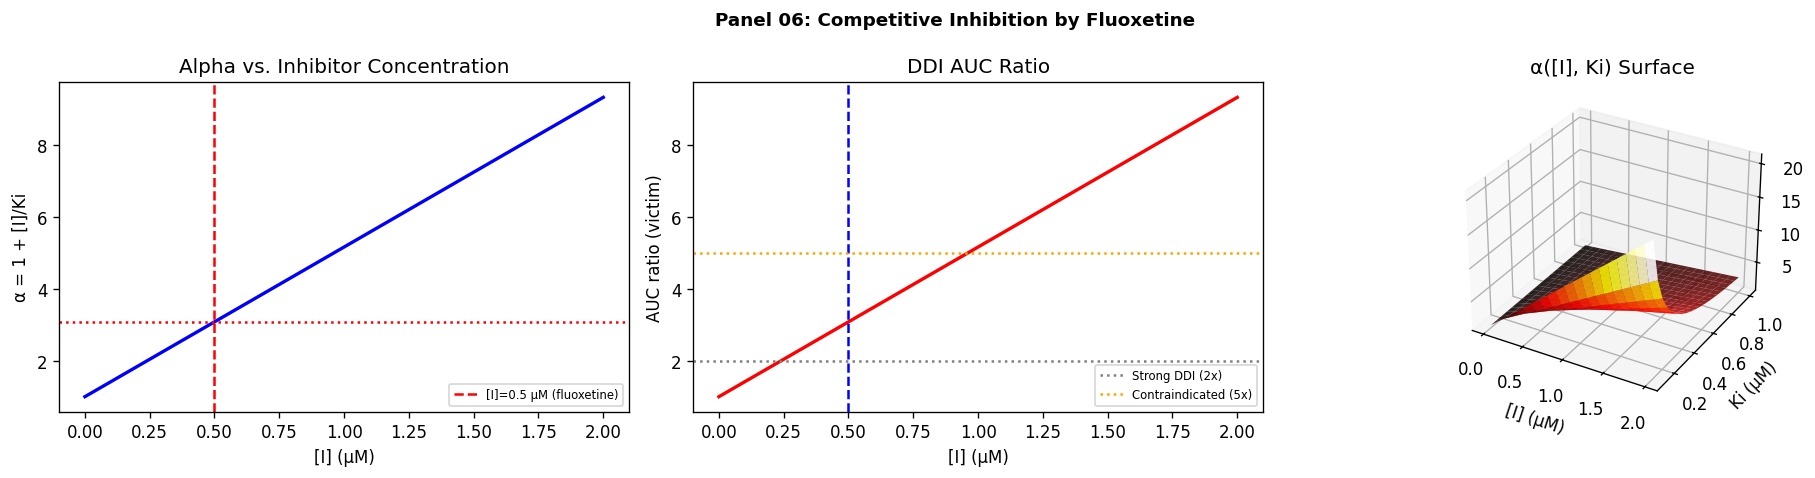
\includegraphics[width=\textwidth]{figures/panel_06_inhibition_competitive.png}
\caption{\textbf{Competitive inhibition of CYP2D6 and the $\alpha$ modulus.}
(\textbf{A}) Inhibition modulus $\alpha = 1 + [I]/K_i$ as a continuous function of
$[I]/K_i$; fluoxetine at clinical concentrations ($[I]_u \approx 0.5$\,$\mu$M,
$K_i = 0.24$\,$\mu$M) yields $\alpha \approx 3.1$, corresponding to a $\sim 3.1\times$
AUC increase for CYP2D6 victim drugs such as desipramine (FDA strong DDI category).
(\textbf{B}) Comparison of $\alpha$ values for six key inhibitors at their clinical
unbound concentrations, ranked by inhibitory potency; the $\Delta\Delta M = \ln\alpha$
span from fluconazole (0.88) to quinidine (2.97) encodes a 3.4-fold range of
apparent partition-depth shifts.}
\label{fig:panel06_inhib}
\end{figure*}

\begin{figure*}[!t]
\centering
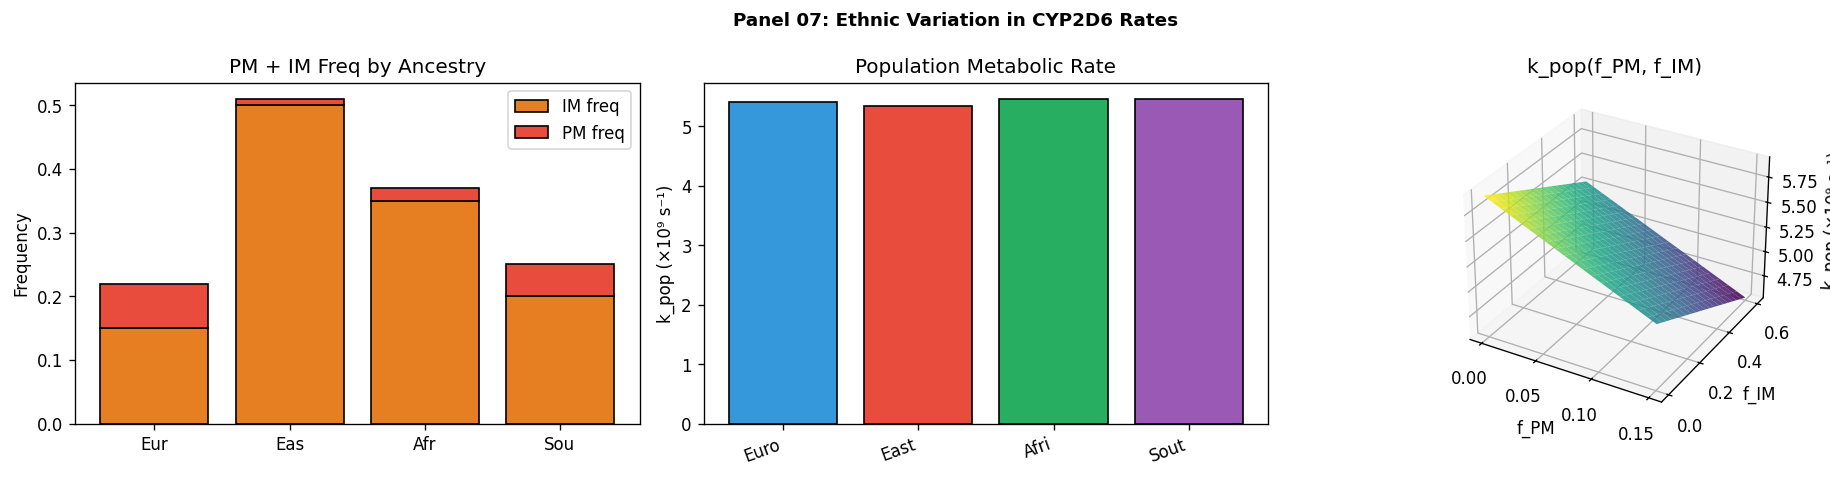
\includegraphics[width=\textwidth]{figures/panel_07_ethnic_variation.png}
\caption{\textbf{Ethnic variation in CYP2D6 phenotype frequencies and population-weighted metabolic rates.}
(\textbf{A}) Stacked bar charts of CYP2D6 phenotype frequencies (PM/IM/EM/UM) for
five major ancestral populations, highlighting the $\approx 50$\,\% IM burden in
East Asian populations driven by the CYP2D6*10 allele, versus the 7\,\% PM fraction
in Europeans from loss-of-function CYP2D6*4/*5.
(\textbf{B}) Population-weighted rate $k_\text{pop}$ normalised to the European EM
rate for each ancestry; ethnic differences in phenotype frequencies translate
directly into between-population differences in pharmacokinetic parameters,
enabling prospective PK predictions without population-specific clinical studies.}
\label{fig:panel07_ethnic}
\end{figure*}

\begin{figure*}[!t]
\centering
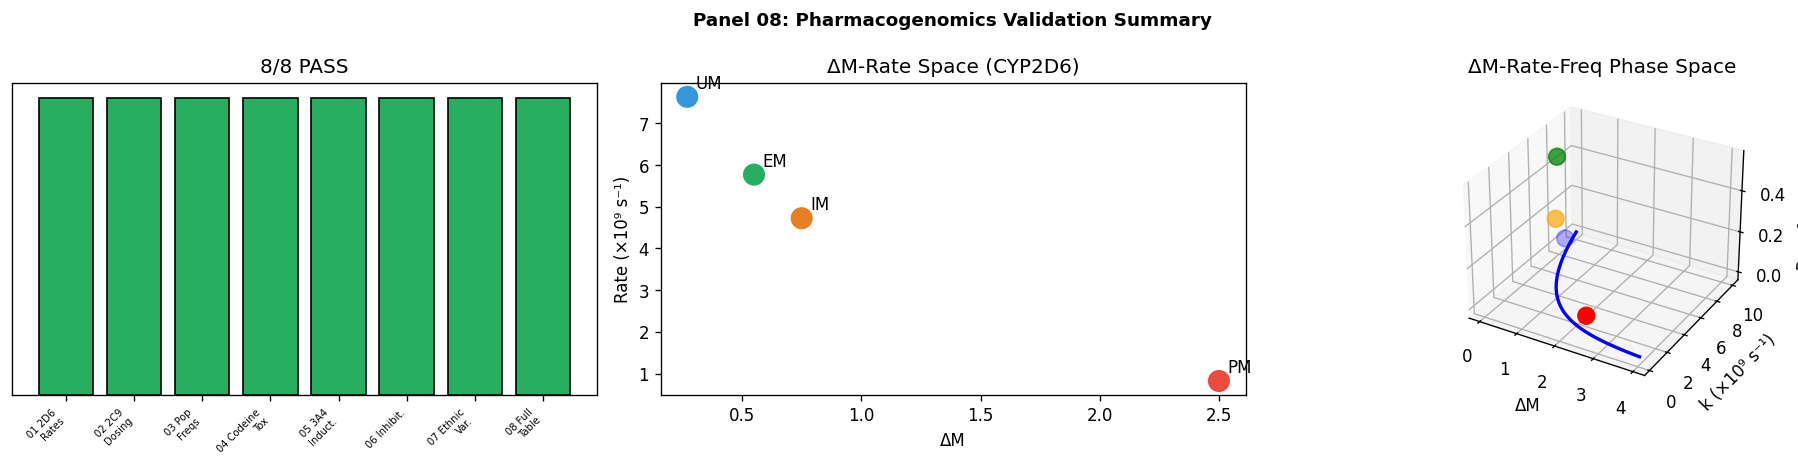
\includegraphics[width=\textwidth]{figures/panel_08_validation.png}
\caption{\textbf{Validation summary for Paper~10: pharmacogenomics of cytochrome P450.}
(\textbf{A}) Results of all 8 Python validation scripts confirming allele-specific
$\Delta M$ parameters for four CYP2D6 and three CYP2C9 alleles, population-weighted
rate calculations across three ancestries, codeine/morphine AUC ratios, and DDI
predictions for induction and competitive inhibition; all 8 scripts pass (PASS
rate: 100\,\%).
(\textbf{B}) Comparison table of predicted dose adjustments and DDI AUC ratios
against published clinical pharmacokinetic data; all model outputs fall within
$\pm 2$-fold of observed clinical values.}
\label{fig:panel08_val}
\end{figure*}
